\chapter{Arbeitspakete}
Die einzelnen Arbeitspakete werden mithilfe des Projektverwaltungstools Redmine
organisiert. Für die Betreuer wurde ein eigener Zugang zum Redmine-Projekt eingerichtet.

\section{Gastzugang Redmine}
http://152.96.192.44/redmine \\
Zugang: guest / zurich2Rapperswil \\

\section{Arbeitspakete}
	\begin{figure}[H]
		%\centering
		% trim=links unten rechts oben
		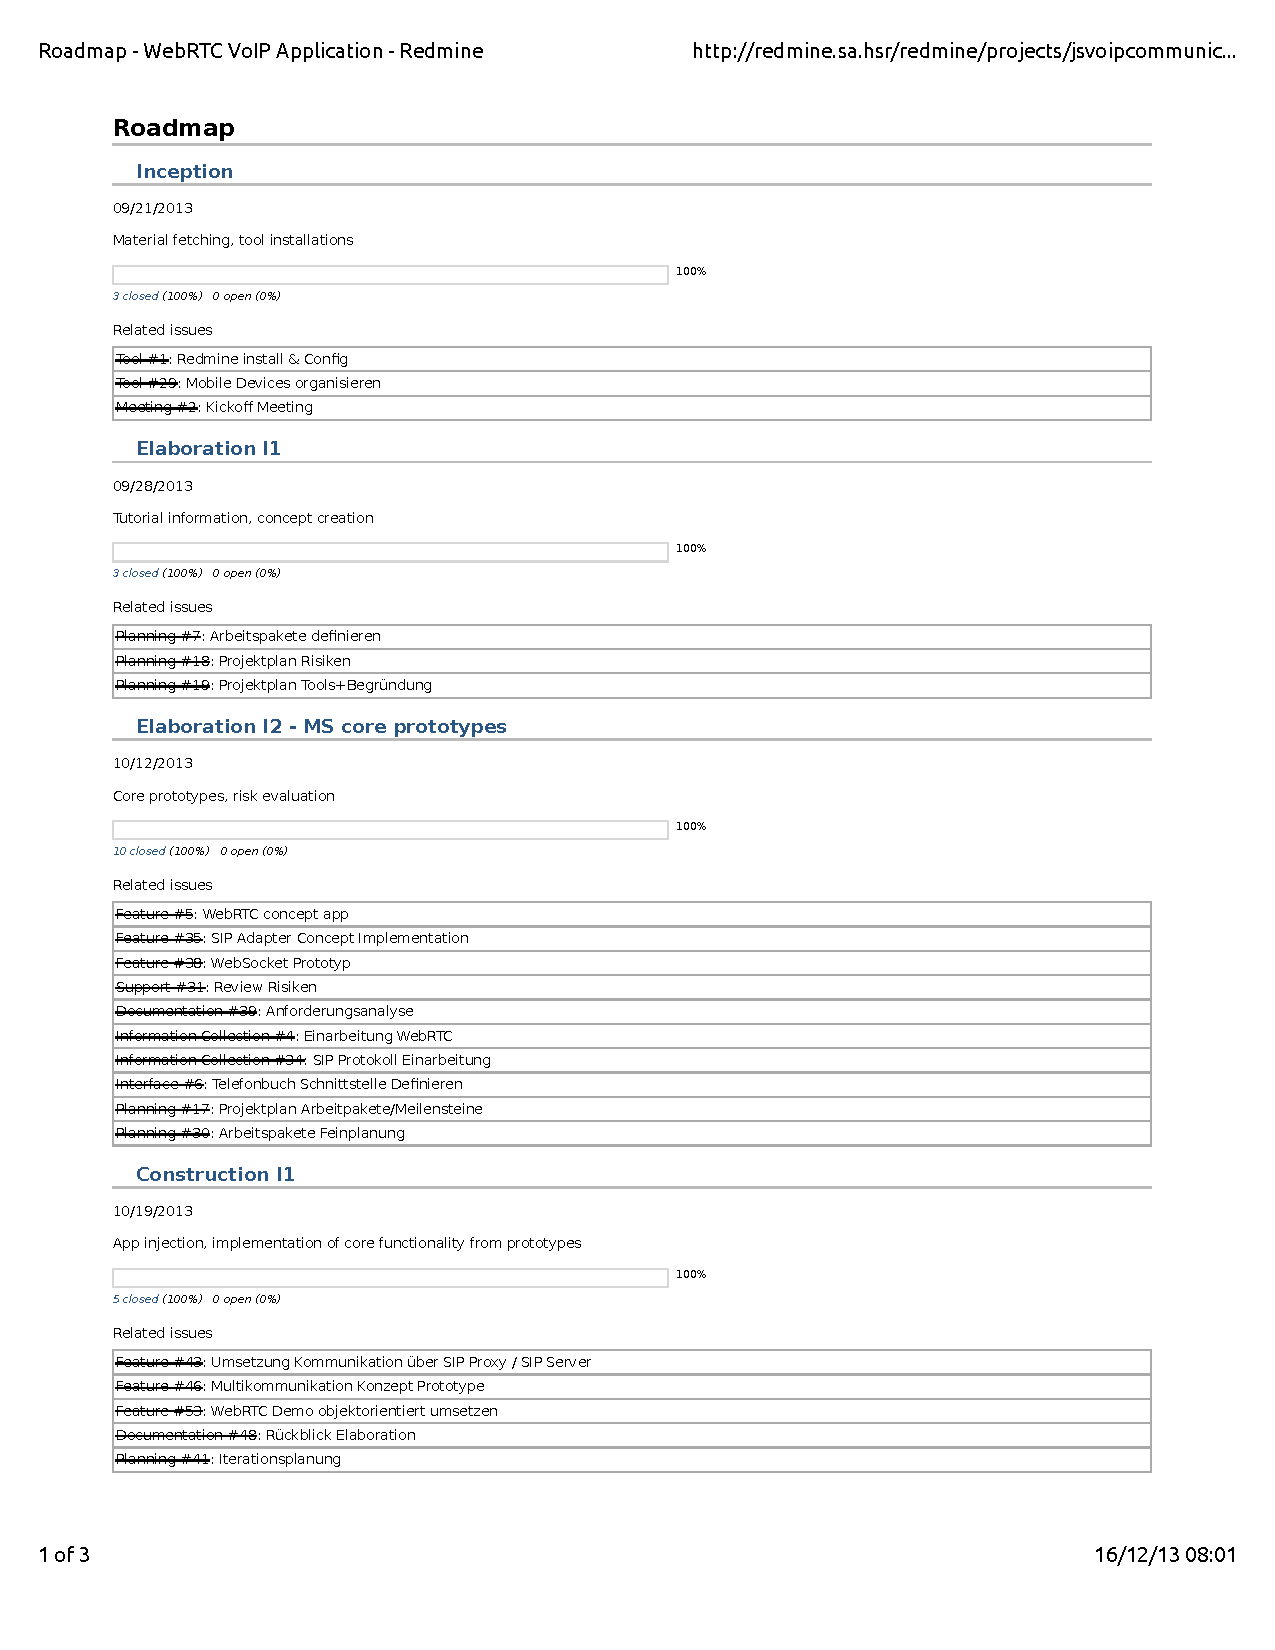
\includegraphics[trim=1.75cm 2cm 2cm 2.5cm, clip=true,page=1,width=0.88\textwidth]{../projektplan/media/roadmap.pdf}
		%\caption[Roadmap]{Arbeitspakete und Milestones}
		%\label{roadmap}
	\end{figure}

	\begin{figure}[H]
		%\centering
		% trim=links unten rechts oben
		\includegraphics[trim=1.75cm 2cm 2cm 2.5cm, clip=true,page=2,width=0.88\textwidth]{../projektplan/media/roadmap.pdf}
		%\caption[Roadmap]{Arbeitspakete und Milestones}
		%\label{roadmap}
	\end{figure}
	
	\subsection{Milestones}
		\subsubsection{Elaboration I2 - MS core prototypes}
			\begin{itemize}
				\item Prototypen der Kernkomponenten, insbesondere der Komponenten mit hohen Risiken
					\begin{itemize}
						\item WebRTC P2P Communication Prototype
						\item SIP Server Connection Prototype
						\item Addressbook Interface Implementation Prototype
						\item Channel Interface Implementation Prototype (XHR Simple Queue Server)
					\end{itemize}
				\item Risikoanalyse
				\item Architekturanalyse
			\end{itemize}
			
		\subsubsection{Construction I2 - MS core functionality}
			\begin{itemize}
				\item Implementation der Kernkomponenten (Prototyp-Komponenten-Elaboration)
					\begin{itemize}
						\item P2P Communication
						\item Channel Reference-Implementation
						\item Addressbook Reference-Implementation
					\end{itemize}
				\item Zwischenstand Projektdokumentation
			\end{itemize}
			
		\subsubsection{Construction I4 - MS final app}
			\begin{itemize}
				\item Implementation der Advanced Komponenten
					\begin{itemize}
						\item Media Scaling
						\item Scallable User Interface
					\end{itemize}
				\item Projektdokumentation
			\end{itemize}
	

	\begin{landscape}
	\subsection{Gantt}
		\begin{figure}[H]
			\centering
			% trim=links unten rechts oben
			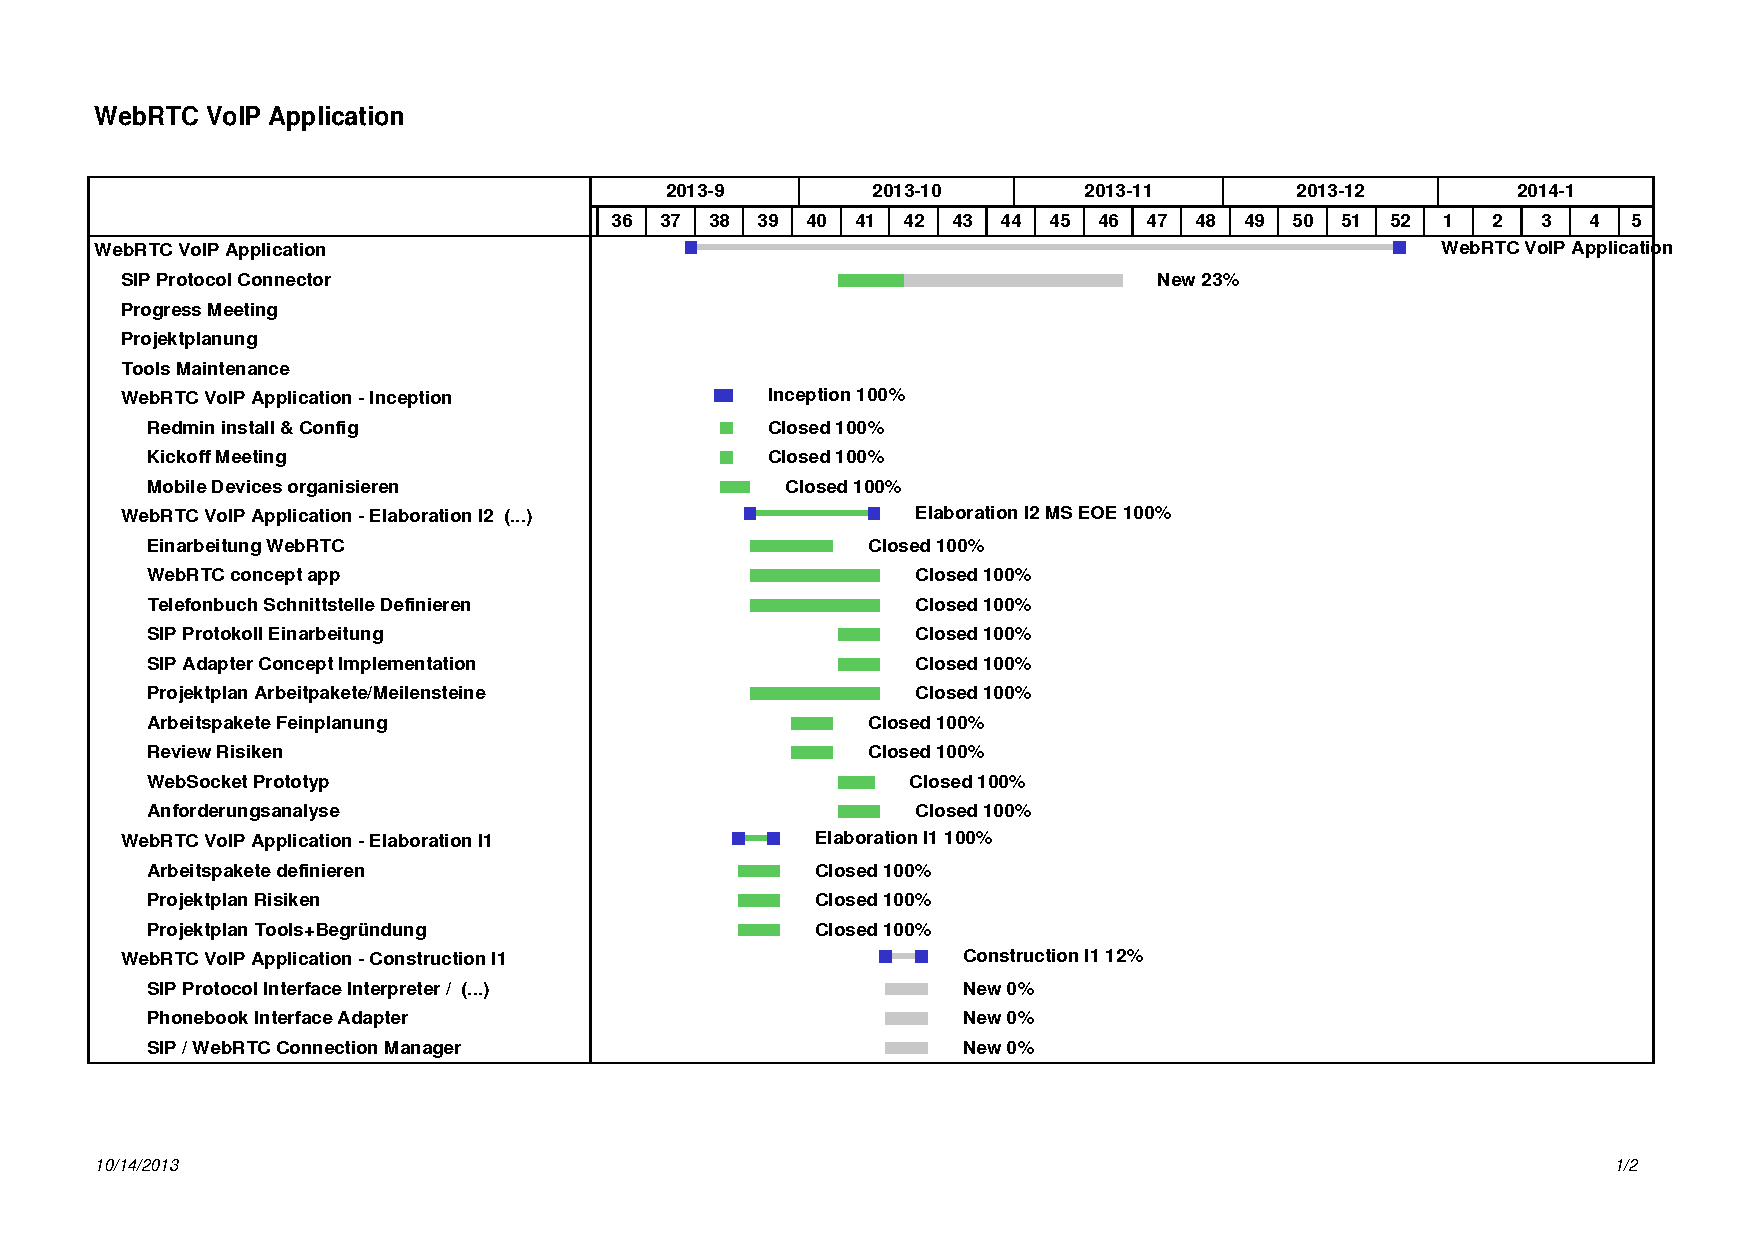
\includegraphics[trim=1.5cm 2.5cm 1cm 3cm, clip=true,page=1,width=1.4\textwidth]{../projektplan/media/jsvoipcommunication-gantt.pdf}
			\caption[Gantt]{Gantt}
			\label{gantt}
		\end{figure}
		\begin{figure}[H]
			\centering
			% trim=links unten rechts oben
			\includegraphics[trim=1.5cm 2.5cm 1cm 1cm, clip=true,page=2,width=1.4\textwidth]{../projektplan/media/jsvoipcommunication-gantt.pdf}
			\caption[Gantt]{Gantt}
			\label{gantt}
		\end{figure}
	\end{landscape}
